%This is a test file to determine the layout of the Owl Datasheet
\documentclass{article}
\pagestyle{myheadings}
\markright{BBa\_K1114211}
\usepackage[xcolor]{mdframed} %Top header has banner!
\usepackage{hyphenat} %Column titles are not to have hyphenation
\usepackage{seqsplit} %Manages long DNA sequence line breaks
\usepackage{ccaption} %Formatting table titles
\usepackage[margin=1in]{geometry} %Setting document margins
\usepackage{graphicx} %Using images
\usepackage{array} %Formatting table size and behavior
\begin{document}
\renewcommand{\topfraction}{0.99} %Helps with keeping whitespace to a minimum
\renewcommand{\textfraction}{0.99}
\renewcommand{\floatpagefraction}{0.99}
\begin{table}[htbp]
\setlength{\belowcaptionskip}{4pt}
\setlength{\extrarowheight}{8pt}
\begin{mdframed}[backgroundcolor=gray!32,topline=false,rightline=false,leftline=false,bottomline=false] \legend{\Huge \underline{BBa\_K1114211}} \end{mdframed} \hfill \break
\begin{tabular}{m{1.2in}m{4.98in}}
\large \textbf{\nohyphens{Part Summary}} & This is a MoClo formatted E1010 RFP gene with CD fusion sites. This is a modified BBa\_E1010 converted to Moclo with one cut site eliminated in the middle of the sequence. This is a Level 0 MoClo part with flanking sites C on the 5' side and site D on the 3' side of the part. The fusion site letters refer to 4bp fusion sites: A = GGAG, B = TACT, C = AATG, D = AGGT, E = GCTT, F = CGCT, G = TGCC, H = ACTA.\\
\large \textbf{\nohyphens{Sequence}} & \seqsplit{aatgatggcttcctccgaggatgttatcaaagagttcatgcgtttcaaagttcgtatggaaggttccgttaacggtcacgagttcgaaatcgaaggtgaaggtgaaggtcgtccgtacgaaggtacccagaccgctaaactgaaagttaccaaaggtggtccgctgccgttcgcttgggacatcctgtccccgcagttccagtacggttccaaagcttacgttaaacacccggctgacatcccggactacctgaaactgtccttcccggaaggtttcaaatgggaacgtgttatgaacttcgaagatggtggtgttgttaccgttacccaggactcctccctgcaagacggtgagttcatctacaaagttaaactgcgtggtaccaacttcccgtccgacggtccggttatgcagaaaaaaaccatgggttgggaagcttccaccgaacgtatgtacccggaggatggtgctctgaaaggtgaaatcaaaatgcgtctgaaactgaaagacggtggtcactacgacgctgaagttaaaaccacctacatggctaaaaaaccggttcagctgccgggtgcttacaaaaccgacatcaaactggacatcacctcccacaacgaggactacaccatcgttgaacagtacgaacgtgctgaaggtcgtcactccaccggtgcttaataaaggt}\\
\large \textbf{\nohyphens{Part Type}} & Basic Part\\
\large \textbf{\nohyphens{Related Parts}} & \seqsplit{E0040m\_CD}\\
\large \textbf{\nohyphens{Pigeon Image}} & \hfill \break 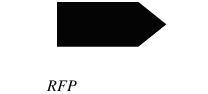
\includegraphics[width=10cm,height=10cm,keepaspectratio]{/Users/Zach/Documents/Owl/igem-datasheet/Datasheet_Generator/src/main/webapp/tmp/1439914923563BBa_K1114211_pigeon.png} \\ 
\large \textbf{\nohyphens{Plasmid Map}} & \hfill \break 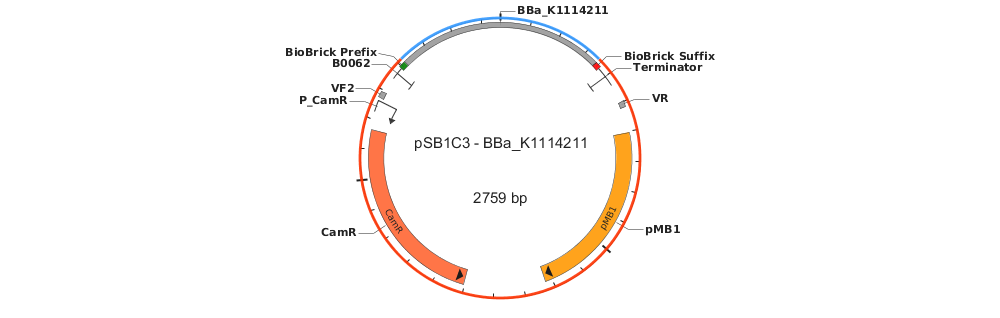
\includegraphics[width=10cm,height=10cm,keepaspectratio]{/Users/Zach/Documents/Owl/igem-datasheet/Datasheet_Generator/src/main/webapp/tmp/1439914923580BBa_K1114211_plasmid_map.png} \
\end{tabular}
\end{table}
\begin{table}[htbp]
\setlength{\belowcaptionskip}{4pt}
\setlength{\extrarowheight}{8pt}
\begin{mdframed}[backgroundcolor=gray!32,topline=false,rightline=false,leftline=false,bottomline=false] \legend{\LARGE Designer Information}\end{mdframed}
\begin{tabular}{m{1.2in}m{4.98in}}
\large \textbf{\nohyphens{Author(s)}} & Traci Haddock\\
\large \textbf{\nohyphens{Date}} & September 7, 2013\\
\large \textbf{\nohyphens{Affiliation}} & Boston University CIDAR Lab\\
\large \textbf{\nohyphens{Team}} & BostonU 2013\\
\large \textbf{\nohyphens{Contact}} & \seqsplit{thaddock@bu.edu}
\end{tabular}
\end{table}
\begin{table}[htbp]
\setlength{\belowcaptionskip}{4pt}
\setlength{\extrarowheight}{8pt}
\begin{mdframed}[backgroundcolor=gray!32,topline=false,rightline=false,leftline=false,bottomline=false] \legend{\LARGE Design Details}\end{mdframed}
\begin{tabular}{m{1.2in}m{4.98in}}
\large \textbf{\nohyphens{Type}} & Coding sequence\\
\large \textbf{\nohyphens{Vector}} & \seqsplit{K1114403}\\
\large \textbf{\nohyphens{Design Components}} & \seqsplit{pSB1C3}
\end{tabular}
\end{table}
\begin{table}[htbp]
\setlength{\belowcaptionskip}{4pt}
\setlength{\extrarowheight}{8pt}
\begin{mdframed}[backgroundcolor=gray!32,topline=false,rightline=false,leftline=false,bottomline=false] \legend{\LARGE Assembly Information}\end{mdframed}
\begin{tabular}{m{1.2in}m{4.98in}}
\large \textbf{\nohyphens{Assembly Method(s)}} & \seqsplit{MoClo}\\
\large \textbf{\nohyphens{Chassis}} & Escherichia coli\\
\large \textbf{\nohyphens{Assembly RFC}} & \seqsplit{94}\\
\large \textbf{\nohyphens{Strain}} & Bioline Alpha- Select Gold\\
\large \textbf{\nohyphens{Scars}} & \seqsplit{yes}
\end{tabular}
\end{table}
\end{document}
